\documentclass{standalone}
\usepackage{tikz}
\begin{document}
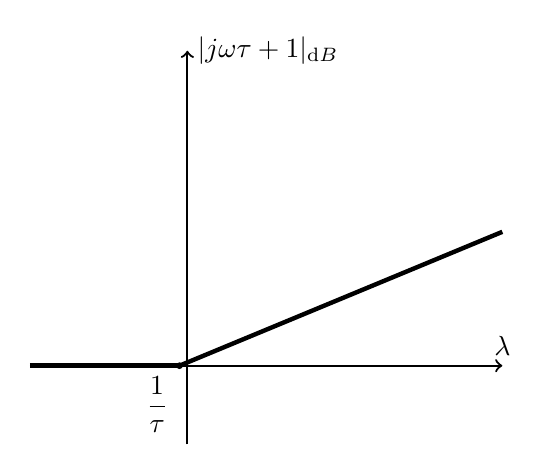
\begin{tikzpicture}[scale=2]
    \draw[->,thick](-1,0)--(2,0)node[above]{$\lambda$};
    \draw[->,thick](0,-0.5)--(0,2)node[right]{$|j\omega\tau+1|_{\mathrm{d} B}$};


    \filldraw[black](-0.05,0)circle(0.5pt);

    \draw[-,ultra thick](-1,0)--(-0.05,0)node[below left]{$\displaystyle\frac{1}{\tau}$};
    \draw[-,ultra thick](-0.05,0)--(2,0.85);
\end{tikzpicture}
\end{document}